\chapter{Simulation der Systemeigenschaften}
\label{chap4}
Ziel dieser Arbeit soll der Vergleich verschiedener Kombinationen von Ladesystem und Speichertechnologie aus technischer Sicht ein. Qualitative Bewertungen einer Kombination sind teilweise ohne Rechnung möglich (z. B. "`\textsc{Primove} ist besser für Lithium-Titanat-Batterien geeignet als für Lithium-Eisenphosphat-Batterien"'). Eine genauere Betrachtung und ein Vergleich von ähnlichen Technologiekombinationen ist jedoch nicht möglich. Daher werden in dieser Arbeit mit Hilfe eines Simulationsmodell quantitative Daten zu den verschiedenen Technologiekombinationen ermittelt.

\section{Simulationsmodell}
%TODO: Ausfüllen
Ausgangspunkt ist ein Elektrobus-Simulationsmodell, das im Fachgebiet Methoden der Produktenwticklung und Mechatronik der TU Berlin entwickelt wurde. Es wurde im Rahmen einer Diplomarbeit von Maximilian Götz erstellt~\cite{Gotz:2013}. Das Modell ist in \textsc{Matlab} und \textsc{simulink} programmiert. Das Modell wird kontinuierlich weiterentwickelt. Für diese Arbeit wurde die Version verwendet, die Tu-Anh Ly am 11. Juni 2015 zur Verfügung stellte. In Abbildung \ref{abb_simmodell} werden die einzelnen Komponenten des Simulationsmodells und ihre Zusammenhänge dargestellt.
\begin{figure}\centering
	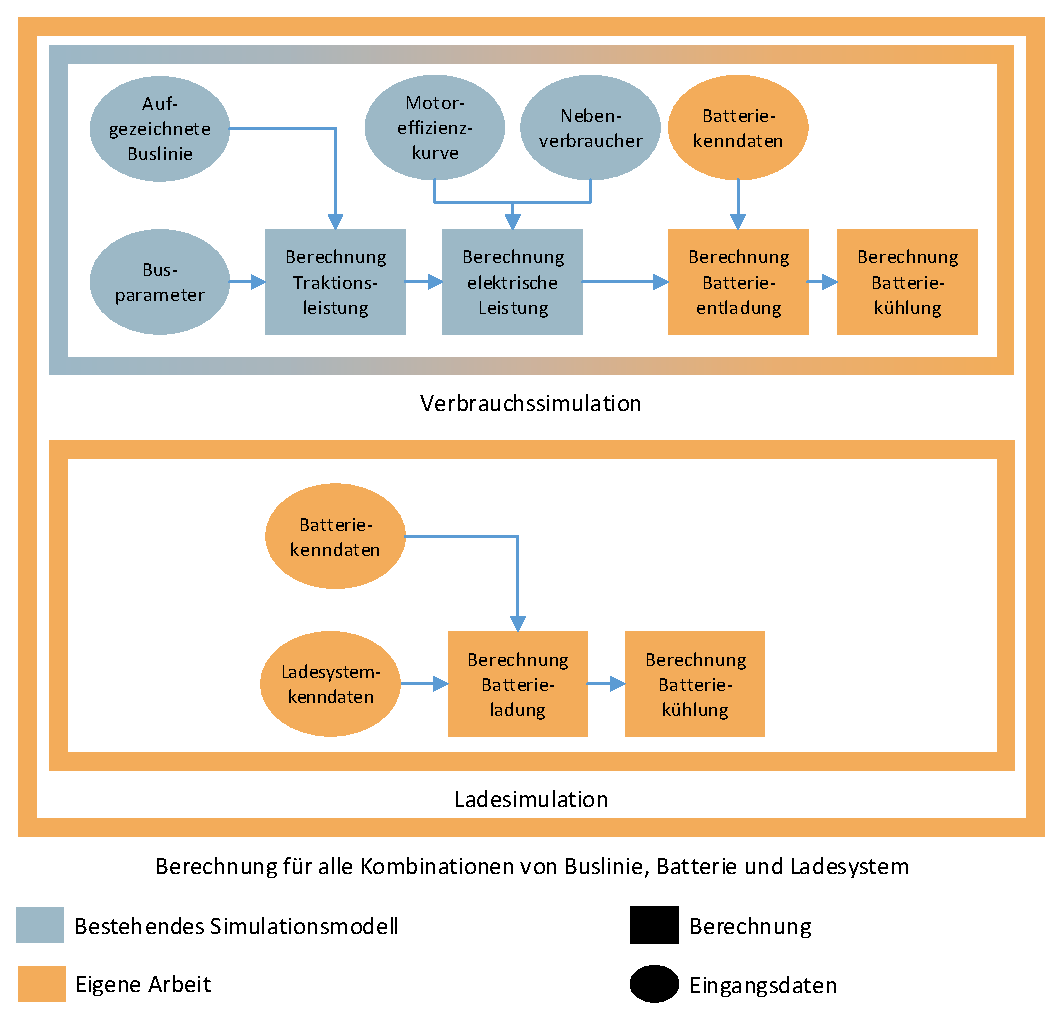
\includegraphics[width=\myFigureWideWidth]{Simulation-Schaubild}
	\caption{Komponenten des Simulationsmodells}
	\label{abb_simmodell}
\end{figure}

\paragraph{Digitaler Anhang} In Anhang \ref{an_Digital} ist eine Kopie des kompletten Simulationsmodells enthalten. Durch Ausführen von \texttt{Simulationsmodell/Batteriesimulation\_Ludger.m} können die Ergebnisse reproduziert werden.

\subsection{Aufgezeichnete Strecke}
Der Energieverbrauch wird anhand einer aufgezeichneten Strecke berechnet. Für jeweils eine Tour wurden dabei Geschwindigkeit, Höhe über dem Meeresspiegel und Passagierzahl mit einer Auflösung von einer Sekunde aufgezeichnet. Die beiden verwendeten Aufzeichnungen sind in Abbildung \ref{Buslinien} zu sehen. Es werden die Buslinien 204 und 192 der BVG betrachtet. Die Buslinie 204 führt vom Bahnhof Zoo zum Südkreuz. Sie ist eine innerstädtische Linie mit niedriger Durchschnittsgeschwindigkeit und vielen Beschleunigungs- und Bremsvorgängen. Die Linie 192 führt vom S-Bahnhof Marzahn zum S-Bahnhof Friedrichsfelde durch den Stadtrand Berlins. Wie in Abbildung \ref{Buslinien} erkennbar ist die Durchschnittsgeschwindigkeit höher und das Geschwindigkeitsprofil gleichmäßiger.
\begin{figure}\centering
	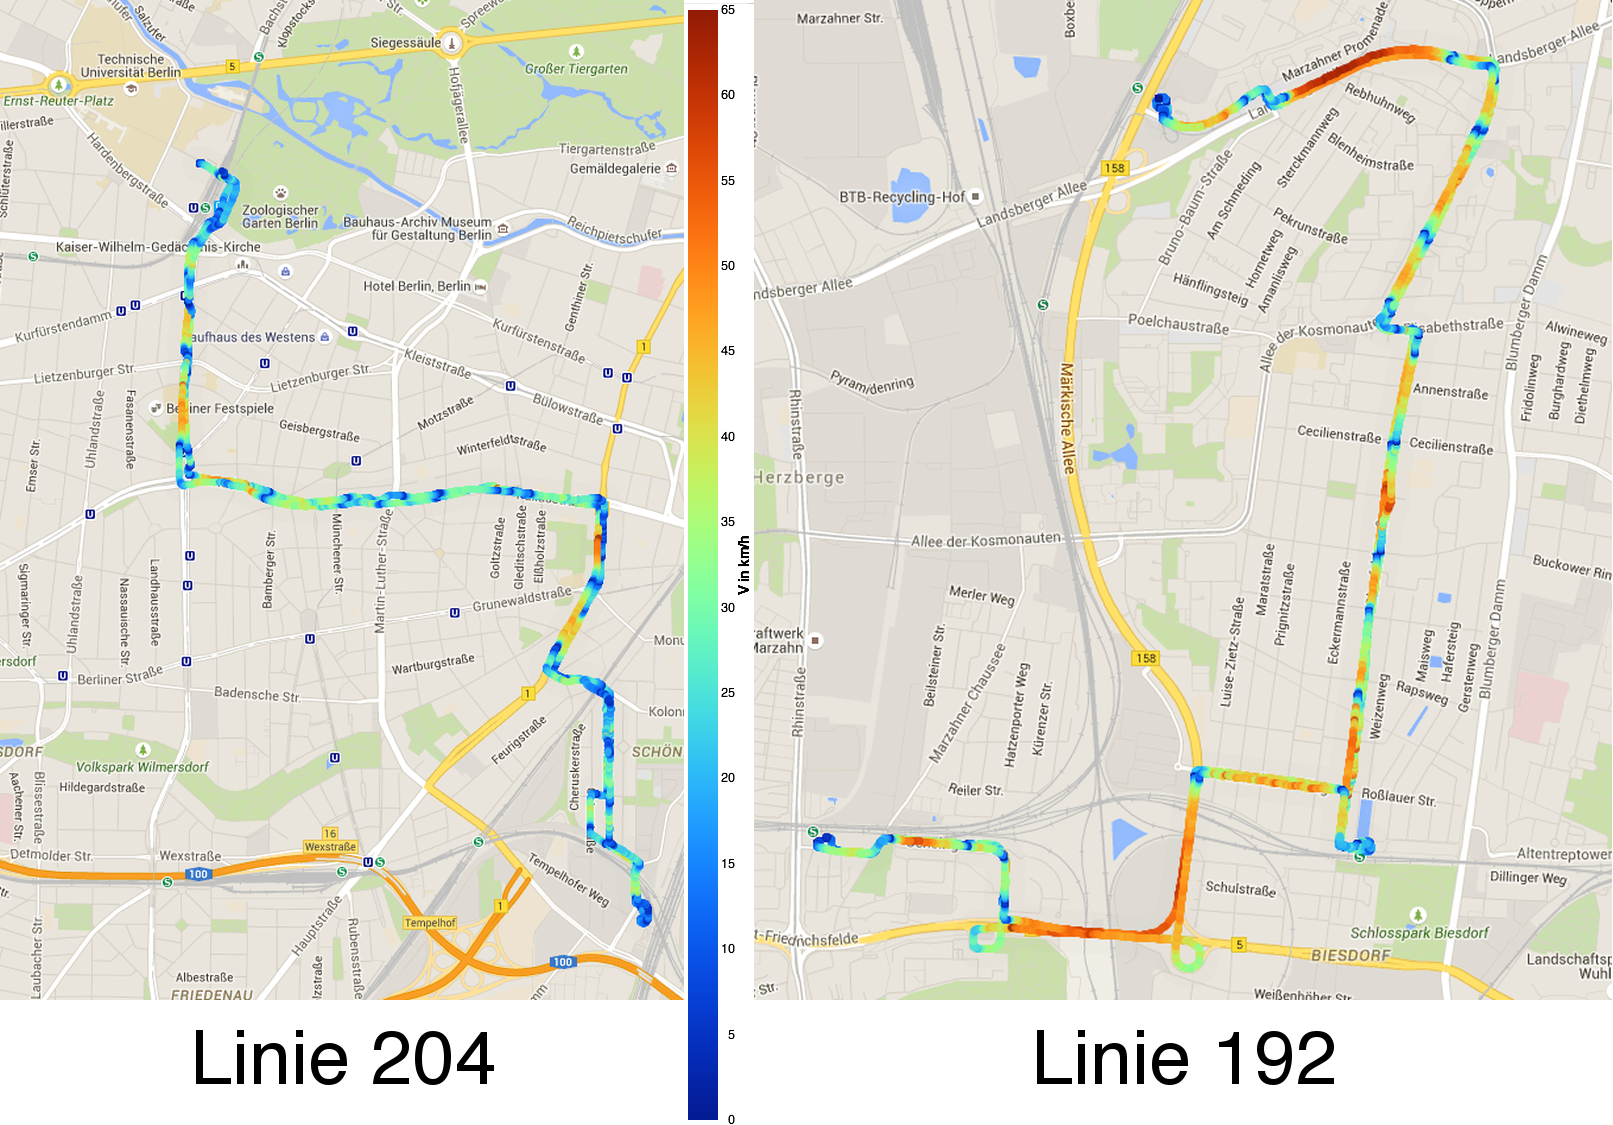
\includegraphics[width=\myFigureWideWidth]{Buslinien}
	\caption[Verlauf und Geschwindigkeitsprofil der Buslinien]{Verlauf und Geschwindigkeitsprofil der Buslinien.}
	\label{Buslinien}
\end{figure}

\subsection{Energieverbrauch}
Über die Strecke sind Beschleunigung, Geschwindgkeit und Steigung zu jedem Zeitpunkt festgelegt. Mit den Busparametern Gewicht, Rollwiderstand, Stirnfläche und $c_w$-Wert werden nun die mechanischen und aerodynamischen Kräfte berechnet, die auf den Bus wirken. Aus diesen Kräften wird die erforderliche Traktionsleistung und Motordrehzahl berechnet.

%TODO: Ausfüllen
Eine von \textbf{xxx} ertellte Effizienzkurve\marginpar{Quelle} berechnet aus Traktionsleistung und Geschwindigkeit die erforderliche elektrische Leistung. In Abbildung \ref{abb_Leistungen} sind die berechneten Leistungen aufgeführt. Die Effizienz des Motors sinkt mit steigender Leistung. Beim Bremsen bei niedrigen Geschwindigkeiten kann die verfügbare Rekuperationsleistung nicht voll ausgenutzt werden.
\begin{figure}\centering
	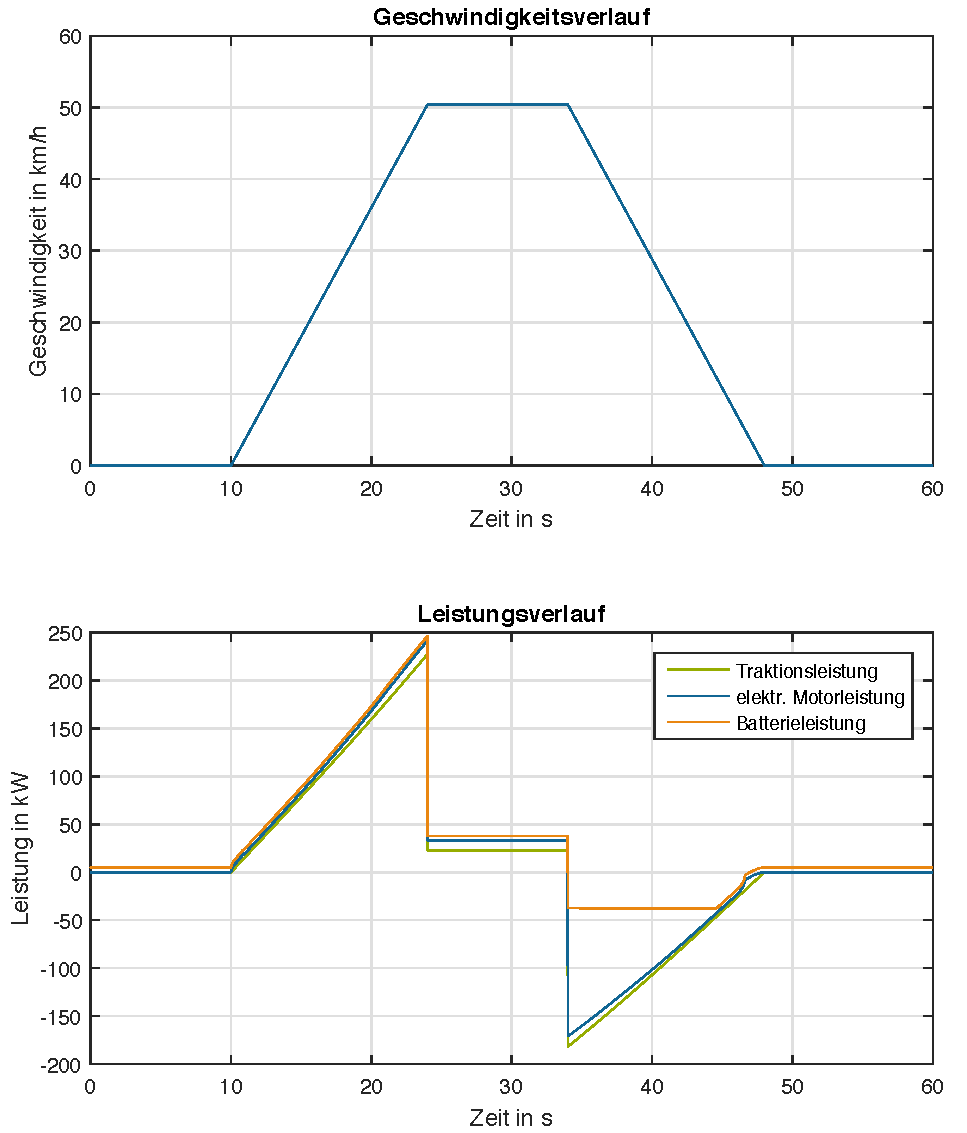
\includegraphics[width=\myFigureWideWidth]{Leistungen}
	\caption[Berechnete Traktions-, Motor- und Batterieleistung]{Berechnete Traktions-, Motor- und Batterieleistung. Es wird Bus mit einer Masse von 13,3 Tonnen konstant mit 1 $\frac{m}{s^2}$ auf 61,2 $\frac{km}{h}$ beschleunigt und nach wenigen Sekunden mit 1 $\frac{m}{s^2}$ bis zum Stillstand abgebremst. Als Batterie wurde hier eine $LiFePO_4$-Batterie gewählt. Durch den maximalen Ladestrom von 1 C ist die Rekuperationsleistung stark begrenzt.}
	\label{abb_Leistungen}
\end{figure}

\subsubsection{Nebenverbraucher}
Neben Antrieb entfällt ein signifikanter Teil der Batterieleistung auf die sogenannten Nebenverbraucher. Der weitaus wichtigste Nebenverbraucher ist die Klimatisierung des Busses. Die Kühlung erfolgt wie in einem Dieselbus durch eine elektrische Klimaanlage mit einer maximalen Dauerleistung von 3 kW an heißen Tagen.

Für die Heizung kann nicht wie bei Dieselbussen die Abwärme des Motors benutzt werden, da der Elektromotor dafür viel zu effizient ist. Im Berliner Elektrobus sollte eine Wärmepumpe verwendet werden. Damit kann mehr Wärme in den Bus transportiert werden als elektrsiche Energie aufgewandt wird. Aufgrund von mangelnder Zuverlässigkeit wird aktuell eine direkte Heizung mit einer Leistung von durchschnittlich 10 kW an kalten Tagen verwendet. Es ist damit zu rechnen, das neue Elektrobusse auch eine Wärmepumpe zur Heizung verwenden werden. Daher wurde die Heiz- und Kühlleistung mit 3 kW abgeschätzt.

Für die anderen Nebenverbraucher wie Licht, Türen und Druckluft wird eine durchschnittliche Leistung von insgesamt 2 kW veranschlagt.

\subsection{Batteriemodell}
Da der Stromverbrauch durch die elektrische Motorleistung und die Nebenverbraucher festgelegt ist, \emph{muss} die Batterie die geforderte Fahrleistung liefern. Sie \emph{kann} bis zu ihrer maximalen Ladeleistung Rekuperationsenergie nutzen. Darüber hinaus anfallende Bremsenergie wird in der Realität über einen Bremswiderstand auf dem Dach abgeleitet, in der Simulation wird sie ignoriert.

In dieser Arbeit wird das empirische Batteriemodell von Tremblay und Dessaint verwendet \cite{tremblay2009experimental}. Dieses generische Batteriemodell liefert weniger exakte Daten als spezialisierte Modelle, kann aber dafür verschiedene Batterietypen darstellen. Ein großer Vorteil dieses Modells ist, das sich die Parameter der aus den Datenblättern der Batterien ablesen lassen. Damit kann man das Modell verschiedenen Batterietypen anpassen, ohne die Batterien selbst zu vermessen.

In Abbildung \ref{abb_Leistungen} ist neben Traktions- und Motorleistung auch die Batterieleistung aufgeführt. Die Leistung ist im Vergleich zur maximalen Motorleistung sehr klein. Deutlich ist hingegen die begrenzte Rekuperationsfähigkeit der Batterie zu sehen.

\subsubsection{Dimensionierung}
Die simulierte Batterie ist aus mehreren Zellen zusammengesetzt\footnote{Diese Zellen entsprechen nicht unbedingt einer chemischen Batteriezelle, sondern der kleinsten Batterie, die einzeln verfügbar ist.}. Durch iterative Optimierung wird die niedrigst mögliche Zellenzahl festgestellt. Als Randbedingung für die Optimierung wird ein maximaler und minimaler Ladezustand der Batterie verwendet. Daneben darf der maximale Entladestrom laut Datenblatt nicht überschritten werden.

\subsubsection{Ladesystem}
Im Simulationsmodell von Götz ist die Ladezeit durch die aufgezeichnete Strecke festgelegt und nicht variabel. Da in dieser Arbeit die Ladezeiten verschiedener Technologiekombinationen verglichen werden sollen, wurde ein separates Modell für den Ladevorgang erstellt. Es besteht aus dem Batteriemodell und einer Energiequelle, die nach einer Totzeit die maximale Ladeleistung bereitstellt. Die Batterie nimmt entsprechend ihrer Ladekurve diese Leistung teilweise oder vollständig auf. Wenn die Batterie den gewünschten Ladezustand erreicht hat, endet die Simulation und die Ergebnisse können entnommen werden.

\subsection{Wärmeberechnung}
Der Abtransport der an der Batterie entstehenden Wärme stellt eine große Herausforderung bei der Auslegung eines Speichersystems dar. Durch Überhitzung kann die Batterie zerstört werden. Aber auch zulässige, jedoch innerhalb des Batteriepacks unterschiedliche Temperaturen führen zu einer unterschiedlichen Lebensdauer der verschiedenen Zellen und reduzieren so die Gesamtlebensdauer. Von daher wird in dieser Simulation auch die Größe des erforderlichen Kühlsystems abgeschätzt.

Wie in Abschnitt \ref{sec_waermeverluste} erläutert überwiegt bei hohen Strömen die vom Innenwiderstand verursachte irreversible Erwärmung. Bei niedrigen Strömen ist der Anteil der reversiblen Erwärmung höher, die Gesamterwärmung jedoch niedriger. Daher wird zur Abschätzung nur der irreversible Anteil mit einem Sicherheitsfaktor von 2 verwendet. Die Erwärmung der Batterien wird mit der Batteriemasse aus dem entsprechenden Datenblatt und den von Pesaran ermittelten Wärmekapazitäten berechnet~\cite{pesaran2001battery}.

Es wird eine parallele Luftkühlung modelliert, bei der die jeweils Luft nur an einer Zelle vorbeigeführt wird. Diese Methode wird von Pesaran als einfache Möglichkeit für eine gleichmäßige Temperatur im Batteriepack empfohlen~\cite{pesaran2001battery}. Es wird angenommen, das die Hälfte der Temperaturdifferenz zwischen Batterie und Umgebungsluft zur Kühlung verwendet werden kann. Als Umgebungstemperatur wird ein Wert von 40 $^{\circ}C$ angenommen, der noch eine kleine Reserve zur höchsten in Berlin gemessenen Temperatur von 38,1 $^{\circ}C$ bietet\cite{tempRekord}. Die benötigte Luftmenge wird durch einem PI-Regler berechnet und der Höchstwert in $\frac{g}{s}$ angegeben.

Es wird nicht unbedingt die ideale Kühlung für jede mögliche Batterie berechnet, sondern es werden vergleichbare Werte für verschiedene Batterien ermittelt, in denen Masse, Wärmekapazität und Maximaltemperatur zusammengefasst sind.

\section{Ergebnisse}
Die folgenden Ausgabedaten der Simulation wurden ausgewählt, um die Kombinationen von Lade- und Speichersystem zu vergleichen:
\begin{description}
	\item[Batteriemasse] Einheit: $kg$
	\item[Batterievolumen] Einheit: $l$
	\item[Kühlluftmasse] Einheit: $\frac{g}{s}$
	\item[Energieverbrauch] Einheit: $\frac{kWh}{km}$
	\item[Zeiteffizienz] Der Anteil der Ladezeit an der Summe von Fahr- und Ladezeit. Kleinere Werte sind besser.
	Einheit: $1$ bei Gelegenheitsladung, h bei Nachtladung
	\item[Ladezyklen pro Kilometer] Mit diesem Wert kann der Einfluss dieser Kombination auf die Lebensdauer der Batterie abgeschätzt werden.
	Einheit: $1$
\end{description}

In den Wertetabellen werden Kurznamen für Batterien und Ladesysteme verwendet. Diese werden in Tabelle \ref{batNamen} und \ref{ladeNamen} erläutert.

\begin{table}\centering
	\begin{tabularx}{\textwidth}{XXXl}
		\toprule
		Kurzname & Hersteller        & Bezeichnung     & Technologie      \\ \midrule
		18650    & Panasonic         & NCR18650B       & $LiNi_xCo_xAl_x$ \\
		Bleiakku & Panasonic         & EC-FV1260       & $PbSO_4$         \\
		LiTiO    & Bombardier        & primove Battery & $Li_4Ti_5O_{12}$ \\
		LFP-HE   & Europen Batteries & EV 45 Ah        & $LiFePO_4$       \\
		LFP-HP   & EIG               & ePLB F 14 Ah    & $LiFePO_4$       \\ \bottomrule
	\end{tabularx}
	\caption{Kurznamen der Batterien}
	\label{batNamen}
\end{table}

\begin{table}\centering
	\begin{tabularx}{\textwidth}{XXXl}
		\toprule
		Kurzname & Hersteller        & Bezeichnung     & Technologie      \\ \midrule
		40kW    & \emph{mehrere}         & IEC 62196-2       & konduktiv-manuell \\
		200kW & Bombardier         & primove       & induktiv         \\
		375kW    & Schunk        & Smart Charging & konduktiv-automatisch \\
		Swap   & k.A.  & k. A.       & Batteriewechsel    \\ \bottomrule
	\end{tabularx}
	\caption{Kurznamen der Ladesystene}
	\label{ladeNamen}
\end{table}

\subsection{Linie 204}
\subsubsection{Nachtladung}
\label{erkl204nacht}
Bei der Ladestrategie "`Nachtladung"' fährt der Bus tagsüber ohne Zwischenladen auf der Strecke. Er absolviert 11 Touren mit einer Gesamtlänge von 132 km. Die Batterie darf sich dabei auf maximal 10\% Ladezustand entladen. Nach Betriebsschluss wird der Bus über Nacht im Depot auf 100\% Ladezustand geladen. Als Ladesystem wurde ein konduktiv-manuelles System mit 40 kW gewählt. Die Ergebnisse sind in Tabelle \ref{204nacht} aufgeführt.

\begin{table}\centering
	\begin{tabulary}{\textwidth}{lrrRRRR}
		\toprule
		Batterie & Masse & Volumen & Kühlluftmasse & Energieverbrauch & Zeiteffizienz & Ladezyklen pro Kilometer \\
		         & $kg$  & $l$     & $\frac{g}{s}$  & $\frac{kWh}{km}$  & $h$           & $1$                      \\ \midrule
		   18650 & 681   & 246     & 1673           & 1,20              & 4,7           & 0,006                   \\
		Bleiakku & 8217  & 3082    & 512            & 1,91              & 9,5           & 0,006                   \\
		   LiTiO & 2174  & 1522    & 190            & 1,26              & 4,9           & 0,006                   \\
		  LFP-HE & 1214  & 736     & 5254           & 1,16              & 4,0           & 0,006                   \\
		  LFP-HP & 1577  & 824     & 4941           & 1,24              & 5,0           & 0,006                   \\ \bottomrule
	\end{tabulary}
	\caption{Simulationsergebnisse Nachtladung Linie 204}
	\label{204nacht}
\end{table}

\subsubsection{Gelegenheitsladung}
\label{erkl204gel}
Bei der Ladestrategie "`Gelegenheitsladung"' wird der Bus nach jeder Folge von Hin- und Rückfahrt aufgeladen. Die Länge einer Tour beträgt 12 km. 

Beim schnellen Laden können die Ladezustände der einzelnen Zellen nicht angeglichen werden, so dass sie über den Betriebstag immer weiter divergieren. Zum Schutz gegen Tiefentladung und Überladung einzelner Zellen wird die Batterie zwischen 30\% und 70\% Ladezustand betrieben.

Bei dieser Ladestrategie werden sämtliche Ladesysteme betrachtet. Die Ergebnisse sind in den Tabellen \ref{204_a} bis \ref{204_e} aufgeführt.

\begin{table}
	\begin{minipage}{0.48\textwidth}
		\centering
		\begin{tabulary}{\linewidth}{lRRRR}
			\multicolumn{5}{c}{Batteriemassen in $kg$}   \\ \toprule
			Bat./LS  & 40kW & 200kW & 375kW &     Swap   \\ \midrule
			18650    &  197 &   200 &   198 &      197   \\
			Bleiakku & 1663 &  1704 &  1667 &     1660   \\
			LiTiO    &  499 &   505 &   501 &      498   \\
			LFP-HE   &  291 &   293 &   291 &      290   \\
			LFP-HP   &  387 &   390 &   388 &      386   \\ \bottomrule
		\end{tabulary}
		\caption{Batteriemassen Linie 204 Gelegnheitsladung}
		\label{204_a}
		\begin{tabulary}{\linewidth}{lRRRR}
			         &      &       &       &  \\
			\multicolumn{5}{c}{Kühlbedarf in $\frac{g}{s}$}  \\ \toprule
			Bat./LS  & 40kW & 200kW & 375kW &          Swap   \\ \midrule
			18650    &  305 &   299 &   300 &           340   \\
			Bleiakku & 1397 &  1367 &  1401 &          1393   \\
			LiTiO    &  631 &  1358 &  1349 &          1343   \\
			LFP-HE   & 5670 &  5720 &  5683 &          5658   \\
			LFP-HP   & 4333 &  4369 &  4342 &          4324   \\ \bottomrule
		\end{tabulary} 
		\caption{Kühlungsbedarf Linie 204 Gelegenheitsladung}
		
		\begin{tabulary}{\linewidth}{lRRRR}
			         &      &       &       &  \\
			\multicolumn{5}{c}{Anteil Ladezeit an Gesamtzeit} \\ \toprule
			Bat./LS  & 40kW & 200kW & 375kW &            Swap \\ \midrule
			18650    & 0,35 &  0,35 &  0,35 &            0,08 \\
			Bleiakku & 0,60 &  0,60 &  0,60 &            0,08 \\
			LiTiO    & 0,24 &  0,10 &  0,10 &            0,08 \\
			LFP-HE   & 0,26 &  0,23 &  0,23 &            0,08 \\
			LFP-HP   & 0,38 &  0,37 &  0,37 &            0,08 \\ \bottomrule
		\end{tabulary} 
		\caption{Ladezeitanteil Linie 204 Gelegenheitsladung}
		
	\end{minipage}\hfill
	\begin{minipage}{0.48\textwidth}
		\centering
		\begin{tabulary}{\linewidth}{lRRRR}
			\multicolumn{5}{c}{Batterievolumina in $l$} \\ \toprule
			Bat./LS  & 40kW & 200kW & 375kW &      Swap \\ \midrule
			18650    &   71 &    72 &    72 &        71 \\
			Bleiakku &  624 &   639 &   625 &       622 \\
			LiTiO    &  349 &   353 &   350 &       348 \\
			LFP-HE   &  176 &   178 &   177 &       176 \\
			LFP-HP   &  202 &   204 &   202 &       202 \\ \bottomrule
		\end{tabulary}
		\caption{Batterievolumina Linie 204 Gelegenheitsladung}
		
		\begin{tabulary}{\linewidth}{lRRRR}
			         &      &       &       &  \\
			\multicolumn{5}{c}{Energieverbrauch in $\frac{kWh}{km}$} \\ \toprule
			Bat./LS  & 40kW & 200kW & 375kW &                   Swap \\ \midrule
			18650    & 1,48 &  1,56 &  1,48 &                   1,47 \\
			Bleiakku & 1,91 &  2,00 &  1,91 &                   1,90 \\
			LiTiO    & 1,24 &  1,39 &  1,33 &                   1,32 \\
			LFP-HE   & 1,39 &  1,46 &  1,40 &                   1,39 \\
			LFP-HP   & 1,48 &  1,57 &  1,49 &                   1,49 \\ \bottomrule
		\end{tabulary} 
		\caption{Energieverbrauch Linie 204 Gelegenheitsladung}
		
		\begin{tabulary}{\linewidth}{lRRRR}
			         &       &       &       &  \\
			\multicolumn{5}{c}{Ladezyklen pro Kilometer} \\ \toprule
			Bat./LS  &  40kW & 200kW & 375kW &      Swap \\ \midrule
			18650    & 0,026 &   0,026 &   0,026 &     0,026 \\
			Bleiakku & 0,031 &   0,030 &   0,031 &     0,031 \\
			LiTiO    & 0,026 &   0,026 &   0,026 &     0,026 \\
			LFP-HE   & 0,031 &   0,031 &   0,031 &     0,031 \\
			LFP-HP   & 0,031 &   0,031 &   0,031 &     0,031 \\ \bottomrule
		\end{tabulary} 
		\caption{Ladezyklen pro Kilometer Linie 204 Gelegenheitsladung}	
		\label{204_e}
		%TODO: WERTE!!!
	\end{minipage}
\end{table}
\subsection{Linie 192}
\subsubsection{Nachtladung}
Die Parameter sind wie in Abschnitt \ref{erkl204nacht} gewählt, allerdings beträgt die Gesamtlänge hier 215 km.

\begin{table}\centering
	\begin{tabulary}{\textwidth}{lrrRRRR}
		\toprule
		Batterie & Masse & Volumen & Kühl-luftmasse & Energie-verbrauch & Zeiteffizienz & Ladezyklen pro Kilometer \\
		         &  $kg$ &     $l$ &  $\frac{g}{s}$ &  $\frac{kWh}{km}$ &           $h$ &                      $1$ \\ \midrule
		18650    &   808 &     293 &           2186 &              0,92 &           5,4 &                    0,004 \\
		Bleiakku & 11726 &    4398 &            746 &              1,74 &          11,9 &                    0,004 \\
		LiTiO    &  2628 &    1840 &            291 &              0,98 &           5,6 &                    0,004 \\
		LFP-HE   &  1432 &     869 &           5402 &              0,88 &           4,8 &                    0,004 \\
		LFP-HP   &  1893 &     988 &           5486 &              0,96 &           5,8 &                    0,004 \\ \bottomrule
	\end{tabulary}
	\caption{Simulationsergebnisse Linie 192 Nachtladung}
	\label{192nacht}
\end{table}
\subsubsection{Gelegenheitsladung}
Die Parameter sind wie in Abschnitt \ref{erkl204nacht} gewählt, allerdings beträgt die Länge einer Tour 19,5 km.
\begin{table}
	\begin{minipage}{0.48\textwidth}
		\centering
		\begin{tabulary}{\linewidth}{lRRRR}
			\multicolumn{5}{c}{Batteriemassen in $kg$}  \\ \toprule
			Bat./LS  & 40kW & 200kW & 375kW &     Swap  \\ \midrule
			18650    &  215 &   217 &   215 &      214  \\
			Bleiakku & 1944 &  1944 &  1944 &     1944  \\
			LiTiO    &  524 &   529 &   525 &      523  \\
			LFP-HE   &  354 &   357 &   354 &      353  \\
			LFP-HP   &  476 &   488 &   477 &      475  \\ \bottomrule
		\end{tabulary} 
		\caption{Batteriemassen Linie 192 Gelegnheitsladung}
		\label{192_a}
		
		\begin{tabulary}{\linewidth}{lRRRR}
			         &      &       &       &  \\
			\multicolumn{5}{c}{Kühlbedarf in $\frac{g}{s}$}   \\ \toprule
			Bat./LS  & 40kW & 200kW & 375kW &          Swap   \\ \midrule
			18650    &  492 &   488 &   486 &           538  \\
			Bleiakku & 1291 &  1324 &  1299 &          1283   \\
			LiTiO    &  776 &  1470 &  1461 &          1456   \\
			LFP-HE   & 6582 &  6639 &  6597 &          6568   \\
			LFP-HP   & 4950 &  4944 &  4960 &          4940   \\ \bottomrule
		\end{tabulary} 
		\caption{Kühlungsbedarf Linie 192 Gelegenheitsladung}
		
		\begin{tabulary}{\linewidth}{lRRRR}
			         &      &       &       &  \\
			\multicolumn{5}{c}{Anteil Ladezeit an Gesamtzeit} \\ \toprule
			Bat./LS  & 40kW & 200kW & 375kW &            Swap \\ \midrule
			18650    & 0,45 &  0,44 &  0,44 &            0,10 \\
			Bleiakku & 0,68 &  0,68 &  0,68 &            0,10 \\
			LiTiO    & 0,33 &  0,15 &  0,15 &            0,10 \\
			LFP-HE   & 0,35 &  0,28 &  0,28 &            0,10 \\
			LFP-HP   & 0,44 &  0,43 &  0,43 &            0,10 \\ \bottomrule
		\end{tabulary} 
		\caption{Ladezeitanteil Linie 192 Gelegenheitsladung}
		
	\end{minipage}\hfill
	\begin{minipage}{0.48\textwidth}
		\centering
		\begin{tabulary}{\linewidth}{lRRRR}
			\multicolumn{5}{c}{Batterievolumina in $l$} \\ \toprule
			Bat./LS  & 40kW & 200kW & 375kW &      Swap \\ \midrule
			18650    &   78 &    78 &    78 &        77 \\
			Bleiakku &  729 &   729 &   729 &       729 \\
			LiTiO    &  367 &   370 &   368 &       366 \\
			LFP-HE   &  214 &   216 &   215 &       214 \\
			LFP-HP   &  248 &   254 &   249 &       248 \\ \bottomrule
		\end{tabulary}
		\caption{Batterievolumina Linie 192 Gelegenheitsladung}
		
		\begin{tabulary}{\linewidth}{lRRRR}
			         &      &       &       &  \\
			\multicolumn{5}{c}{Energieverbrauch in $\frac{kWh}{km}$} \\ \toprule
			Bat./LS  & 40kW & 200kW & 375kW &                   Swap \\ \midrule
			18650    & 1,22 &  1,23 &  1,22 &                   1,21 \\
			Bleiakku & 1,60 &  2,69 &  1,61 &                   1,60 \\
			LiTiO    & 0,99 &  1,11 &  1,06 &                   1,05 \\
			LFP-HE   & 1,09 &  1,15 &  1,10 &                   1,09 \\
			LFP-HP   & 1,19 &  1,24 &  1,19 &                   1,19 \\ \bottomrule
		\end{tabulary} 
		\caption{Energieverbrauch Linie 192 Gelegenheitsladung}
		
		\begin{tabulary}{\linewidth}{lRRRR}
			         &       &       &       &  \\
			\multicolumn{5}{c}{Ladezyklen pro Kilometer} \\ \toprule
			Bat./LS  &  40kW & 200kW & 375kW &      Swap \\ \midrule
			18650    & 0,020 & 0,020 & 0,020 &     0,020 \\
			Bleiakku & 0,022 & 0,023 & 0,022 &     0,022 \\
			LiTiO    & 0,020 & 0,020 & 0,020 &     0,020 \\
			LFP-HE   & 0,020 & 0,020 & 0,020 &     0,020 \\
			LFP-HP   & 0,020 & 0,020 & 0,020 &     0,020 \\ \bottomrule
		\end{tabulary} 
		\caption{Ladezyklen pro Kilometer Linie 192 Gelegenheitsladung}
		\label{192_e}
	\end{minipage}	
\end{table}